\documentclass{standalone}

\usepackage[dvipsnames]{xcolor}
\usepackage{tikz}
\usepackage{verbatim}
\usetikzlibrary{calc,trees,positioning,arrows,chains,shapes.geometric,%
    decorations.pathreplacing,decorations.pathmorphing,shapes,%
    matrix,shapes.symbols, plotmarks}

 \begin{document}

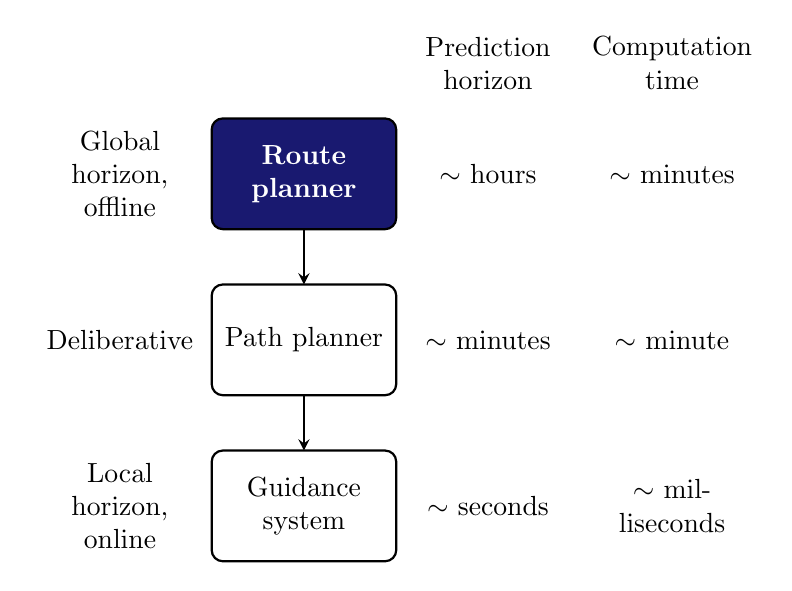
\begin{tikzpicture}[x=6.65em,y=4em]

	\tikzstyle{block} = [rectangle, draw, thick,
    		text width=6em, text centered, rounded corners, minimum height=4em]
	\tikzstyle{block_marked} = [block, fill=MidnightBlue, text=white, font=\bfseries]
	\tikzstyle{plaintext} = [draw=none,fill=none,text width=6em, text centered]
	\tikzstyle{line} = [draw, ->,>=stealth, thick, rounded corners]

    \node [plaintext] at (1, 1) (scope) {Prediction \\ horizon};
    \node [plaintext] at (2, 1) (computation_time) {Computation \\ time};

    % Place nodes
    \node [block_marked] at (0, 0) (route_planner) {Route planner};
    \node [plaintext] at (-1, 0) (route_planner_left) {Global\\horizon, \\ offline};
    \node [plaintext] at (1, 0) {$\sim$ hours};
    \node [plaintext] at (2, 0) {$\sim$ minutes};
    
    \node [block] at (0, -1.5) (path_planner) {Path planner};
    \node [plaintext] at (-1, -1.5) {Deliberative};
    \node [plaintext] at (1, -1.5) {$\sim$ minutes};
    \node [plaintext] at (2, -1.5) {$\sim$ minute};
    
    \node [block] at (0, -3) (path_follower) {Guidance system};
    \node [plaintext] at (-1, -3) (path_follower_left) {Local\\horizon, \\ online};
    \node [plaintext] at (1, -3) {$\sim$ seconds};
    \node [plaintext] at (2, -3) {$\sim$ milliseconds};
    
   % \draw[red,thick,dashed] (-1.75,-0.75) -- (2.75,-0.75) -- (2.75,-2.25) -- (-1.75,-2.25) -- (-1.75,-0.75);
    
    % Draw edges
    \path [line] (0, -0.5) -- (0,-1);
    \path [line] (0, -2) -- (0,-2.5);
\end{tikzpicture}
\end{document}